\documentclass[UTF8]{report}
\usepackage{graphicx}
\usepackage{xetexko}

\title{%
    <컴퓨터프로그래밍 3> 실습 보고서 \\ 
    \large [제 07 주] 성적처리2}
\author{201704150 허강준}
\date{\today}


\begin{document}
    \maketitle
    \tableofcontents

    \chapter{프로그램 설명서}
        본 보고서에서는 성적 처리를 위한 객체를 정의하고 처리하는 프로그램에 대해 기술한다.

        \section{프로그램의 전체 설계 구조 (MVC 등)}
            
            \paragraph{%
                \normalfont 성적 처리 프로그램은 크게 프로그램의 제어를 담당하는 Controller인 \texttt{app\_controller}, 입/출력을 담당하는 View인 \texttt{app\_view}, 그리고 성적 처리를 위한 모델인 \texttt{student}, \texttt{lecture\_view} 등으로 나뉜다. 또한 리스트 처리를 위하여 C++의 Standard Template Library에 정의된 \texttt{vector} Type을 일부 구현하였다.
            }

            \paragraph{%
                \normalfont 큰 틀에서 이전 과제와 크게 다르지 않으나 단순 정수 대신 string을 같이 취급하게 되었으며, STL Library를 간략하게나마 도입하였다.
            }
            
        \section{함수 설명서}
            
            \paragraph{\texttt{VECTOR(type)}}
            \paragraph{%
                \normalfont C++의 Standard Template Library에 정의된 Container Template Type인 \texttt{vector}를 일부 구현하였다. 구현된 메서드는 \texttt{new},  \texttt{delete}, \texttt{at}, \texttt{front}, \texttt{back}, \texttt{data}, \texttt{empty}, \texttt{size}, \texttt{max\_size}, \texttt{clear}, \texttt{insert}, \texttt{erase}, \texttt{push\_back}, \texttt{pop\_back}, \texttt{swap} 이다.
            }

            \paragraph{\texttt{lecture\_class}}
            \paragraph{%
                \normalfont \texttt{VECTOR(student) 의 type alias}
            }

            \paragraph{\texttt{lecture\_class\_sort\_score()}}
            \paragraph{%
                \normalfont lecture\_class내의 student 데이터를 점수별로 정렬하는 함수. Quick Sort Algorithm을 사용함.
            }


            \paragraph{\texttt{lecture\_class\_sort\_qsort()}}
            \paragraph{%
                \normalfont Qucik Sort Algorithm을 이용하여 내부 데이터를 정렬하는 함수
            }

            \paragraph{\texttt{lecture\_class\_sort\_qsort\_rec()}}
            \paragraph{%
                \normalfont Quick Sort Algorithm을 수행하는 재귀 함수
            }

            \paragraph{\texttt{lecture\_class\_sort\_partition()}}
            \paragraph{%
                \normalfont Quick Sort Algorithm의 Partition을 수행하는 함수
            }

            \paragraph{\texttt{lecture\_view\_create()}}
            \paragraph{%
                \normalfont \texttt{lecture\_class} 객체를 기반으로 각종 정보를 제공하는 객체인 \texttt{lecture\_view}를 생성한다.
            }

            \paragraph{\texttt{lecture\_view\_delete()}}
            \paragraph{%
                \normalfont  \texttt{lecture\_view}를 제거한다.
            }

            \paragraph{\texttt{lecture\_view\_list()}}
            \paragraph{%
                \normalfont  \texttt{lecture\_view}내에 저장된 정렬된 리스트 객체를 반환한다.
            }

            \paragraph{\texttt{lecture\_view\_total()}}
            \paragraph{%
                \normalfont  총 학생 수를 반환한다.
            }

            \paragraph{\texttt{lecture\_view\_conv\_grade()}}
            \paragraph{%
                \normalfont  점수를 바탕으로 학점을 반환한다.
            }

            \paragraph{\texttt{lecture\_view\_get\_grade\_count()}}
            \paragraph{%
                \normalfont  인자로 받은 학점에 따라 학생 수를 반환한다.
            }

            \paragraph{\texttt{lecture\_view\_avg()}}
            \paragraph{%
                \normalfont 평균값을 리턴한다. 
            }

            \paragraph{\texttt{lecture\_view\_above\_avg()}}
            \paragraph{%
                \normalfont 평균 이상인 학생의 수를 리턴한다.
            }

            \paragraph{\texttt{lecture\_view\_sum()}}
            \paragraph{%
                \normalfont 총 합계를 리턴한다. \texttt{lecture\_view\_sum\_rec} 을 이용하여 재귀적으로 계산한다.
            }

            \paragraph{\texttt{lecture\_view\_min()}}
            \paragraph{%
                \normalfont 최저 점수를 리턴한다. \texttt{lecture\_view\_min\_rec} 을 이용하여 재귀적으로 계산한다.
            }

            \paragraph{\texttt{lecture\_view\_max()}}
            \paragraph{%
                \normalfont 최고 점수를 리턴한다. \texttt{lecture\_view\_max\_rec} 을 이용하여 재귀적으로 계산한다.
            }

            \paragraph{\texttt{student\_create()}}
            \paragraph{%
                \normalfont \texttt{student} 객체를 생성한다.
            }

            \paragraph{\texttt{student\_delete()}}
            \paragraph{%
                \normalfont \texttt{student} 객체를 제거한다.
            }

            \paragraph{\texttt{student\_get\_student\_id()}}
            \paragraph{%
                \normalfont 현재 객체의 학번을 리턴한다.
            }

            \paragraph{\texttt{student\_get\_score()}}
            \paragraph{%
                \normalfont 현재 객체의 점수를 리턴한다.
            }

            \paragraph{\texttt{student\_is\_id\_valid()}}
            \paragraph{%
                \normalfont 입력된 학번이 형식에 맞는지 검사한다.
            }

            \paragraph{\texttt{student\_is\_score\_valid()}}
            \paragraph{%
                \normalfont 입력된 점수가 범위 내에 있는지 검사한다.
            }

            \paragraph{\texttt{app\_jmp\_env()}}
            \paragraph{%
                \normalfont \texttt{app\_controller\_exit}을 위한 \texttt{jmp\_buf} 객체 리턴용 함수
            }

            \paragraph{\texttt{app\_controller\_create()}}
            \paragraph{%
                \normalfont \texttt{app\_controller} 객체를 생성한다. 명령행 인자 (argc, argv)를 Application Context에 함께 저장한다.
            }

            \paragraph{\texttt{app\_controller\_run()}}
            \paragraph{%
                \normalfont Application Context Main Routine
            }

            \paragraph{\texttt{app\_controller\_exit()}}
            \paragraph{%
                \normalfont 입력된 인자값을 exit code로 하여 Application Context를 종료한다.
            }

            \paragraph{\texttt{app\_controller\_get\_result()}}
            \paragraph{%
                \normalfont Application Context의 Status Code를 반환한다.
            }

            \paragraph{\texttt{app\_controller\_delete()}}
            \paragraph{%
                \normalfont \texttt{app\_controller} 객체를 제거한다.
            }

            \paragraph{\texttt{app\_controller\_get\_input()}}
            \paragraph{%
                \normalfont \texttt{student} 객체를 생성하기 위한 여러 값을 입력받는다.
            }

            \paragraph{\texttt{app\_controller\_input\_is\_valid()}}
            \paragraph{%
                \normalfont 입력된 값이 유효한지 검사한다.
            }

            \paragraph{\texttt{app\_controller\_show\_statistics()}}
            \paragraph{%
                \normalfont 여태까지 입력된 값을 바탕으로 통계 정보를 출력한다.
            }

            \paragraph{\texttt{appview\_err\_invalid\_score()}}
            \paragraph{\texttt{appview\_err\_too\_long\_id()}}
            \paragraph{%
                \normalfont 점수, 학번 관련 오류 메세지를 출력한다.
            }

            \paragraph{\texttt{appview\_getch()}}
            \paragraph{%
                \normalfont 키보드로부터 직접 한 글자를 받아온다.
            }

            \paragraph{\texttt{appview\_in\_get\_continue)}}
            \paragraph{%
                \normalfont 입력을 계속할 것인지 묻고, 해당 질의에 대한 입력을 받는다.
            }

            \paragraph{\texttt{appview\_in\_get\_student()}}
            \paragraph{%
                \normalfont 학생 정보를 입력받는다.
            }

            \paragraph{\texttt{appview\_out\_println()}}
            \paragraph{%
                \normalfont 문자열을 출력한다.
            }

            \paragraph{\texttt{appview\_out\_sorted\_student\_list()}}
            \paragraph{%
                \normalfont 정렬된 학생 목록을 출력한다.
            }

            \paragraph{\texttt{appview\_out\_statistics()}}
            \paragraph{%
                \normalfont 학생 점수 통계를 출력한다.
            }

            \paragraph{\texttt{appview\_out\_student\_info()}}
            \paragraph{%
                \normalfont 학생 정보를 출력한다.
            }

        \section{종합 설명서}

            \paragraph{%
                \normalfont  이번 프로그램은 이전주 프로그램에 특정 학생을 식별할 수 있는 key값(여기서는 학번)을 추가로 입력받아 저장한 뒤, 그 성적을 처리하도록 하는 데 목적이 있다. 또한 더욱 편리한 리스트 처리를 위하여 vector type을 도입하였다.
            }
            
    \chapter{프로그램 장단점/특이점 분석}
            \section{vector type의 사용}
            \paragraph{%
                \normalfont vector 타입은 본래 C++에서 사용되는 표준 라이브러리인 Standard Template Library에 정의된 Container 로써, 타입을 직접 지정하여 힙 공간에 데이터를 저장하고 처리하는 타입이다. 본래 강의 자료에 \texttt{NewVector} 함수가 있는 것에 영감을 받아, 언어의 한계 상 구현이 애매한 요소들을 제외하고, 최대한 실용적으로 사용할 수 있는 메서드들 만을 골라 매크로를 이용하여 구현하였다.
            }   

            \section{\texttt{lecture\_view} Type에 대하여}
            \paragraph{%
                \normalfont \texttt{lecture\_view} 타입은 \texttt{lecture\_class} 타입에 저장된 학생 데이터를 바탕으로 각종 메타데이터를 제공함에 목적을 두는 모델이다. 평균, 총 합계, 최대, 최소, 학점 별 카운팅 등의 기능을 제공하며 내부에 저장된 학생 데이터는 객체 생성 시점에서 정렬되어있다.
            }

    \chapter{실행 결과 분석}
        \section{실행 결과 캡쳐}
        \begin{figure}[!htb]
            \centering
            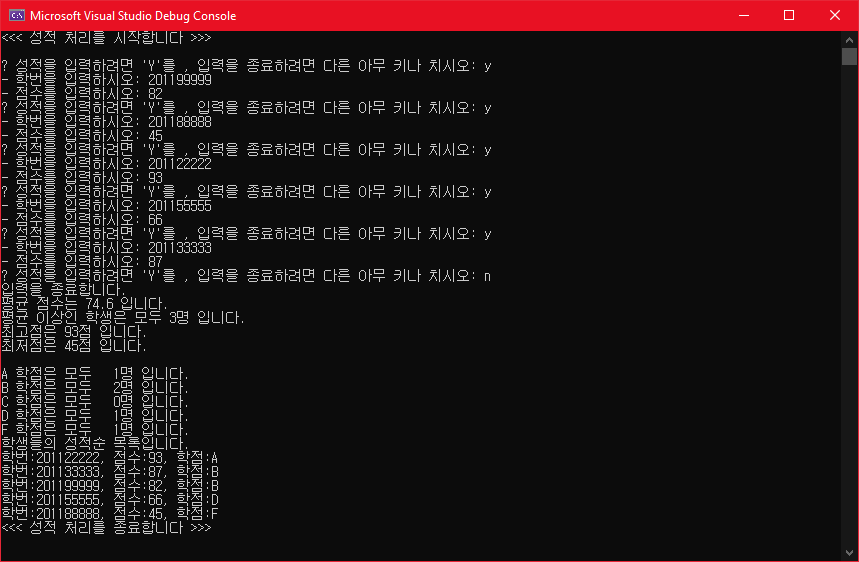
\includegraphics[width=\textwidth]{output_1.png}
            \caption{실행 결과1}
        \end{figure}
        
        \begin{figure}[!htb]
            \centering
            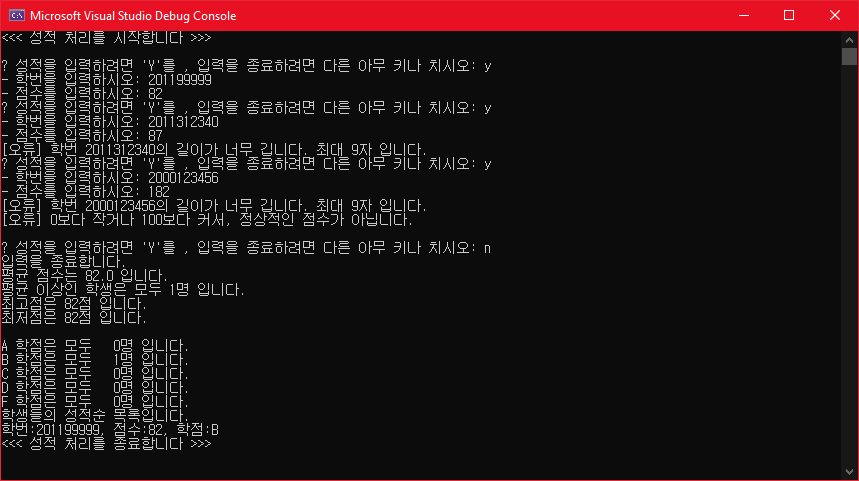
\includegraphics[width=\textwidth]{output_2.png}
            \caption{실행 결과2}
        \end{figure}

        \begin{figure}[!htb]
            \centering
            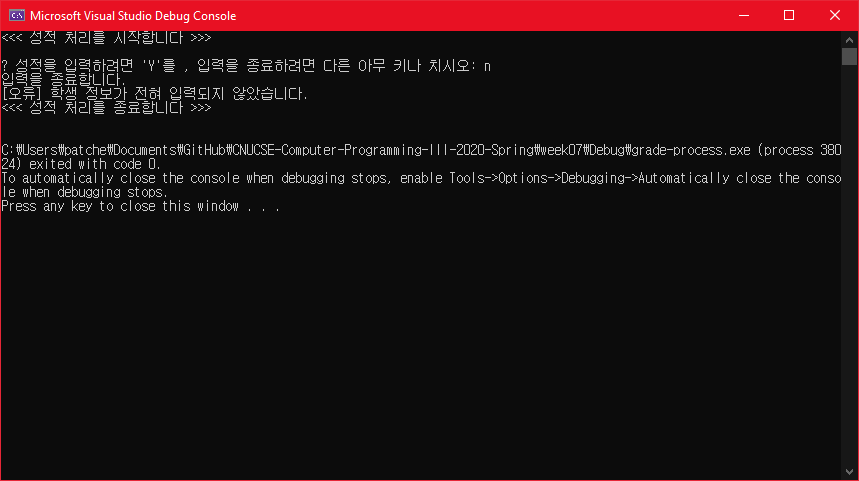
\includegraphics[width=\textwidth]{output_3.png}
            \caption{실행 결과3}
        \end{figure}

        \begin{figure}[!htb]
            \centering
            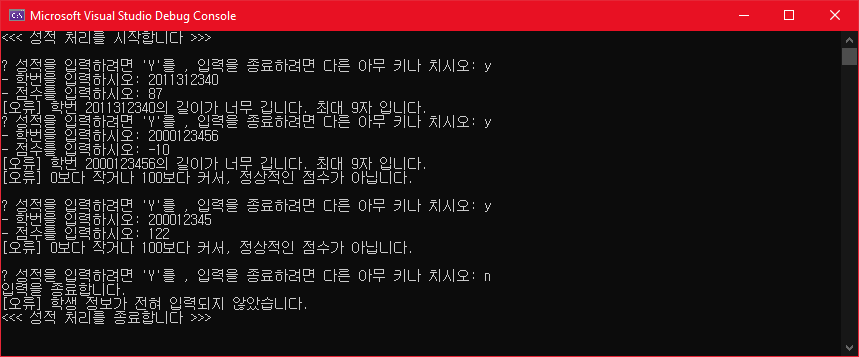
\includegraphics[width=\textwidth]{output_4.png}
            \caption{실행 결과4}
        \end{figure}

        \newpage
        \newpage

        \section{입력과 출력}
            실습 자료에서 제시된 입력을 사용하였으며 출력 결과는 상기한 것과 같았음.
        \section{결과 분석}
            모든 입력에 대하여 정상적인 출력을 확인하였음.

    \chapter{소스코드}
        소스코드는 제출된 압축파일에 같이 동봉되어있으며 GitHub (0x00000FF/CNUCSE-Computer-Programming-III-2020-Spring) 에서도 열람할 수 있다.
\end{document}